\documentclass[tikz,border=5pt]{standalone}
\usepackage{amsmath}
\usetikzlibrary{arrows.meta}
\definecolor{compA}{HTML}{0072B2}
\definecolor{compB}{HTML}{D55E00}
\definecolor{compC}{HTML}{009E73}
\definecolor{compD}{HTML}{CC79A7}

% Each triangle is a fixed rooted component. Its apex is its attachment root.
\newcommand{\fullquartet}[5]{%
 \begin{scope}[xshift=#1cm]
  \draw[tree] (-.38,0)--(.38,0);
  \foreach \x/\y/\id/\col in
    {-1/.55/#2, -1/-.55/#3, 1/.55/#4, 1/-.55/#5}{
   \pgfmathsetmacro{\side}{ifthenelse(\x<0,-.38,.38)}
   \pgfmathsetmacro{\base}{ifthenelse(\y<0,\y-.61,\y+.61)}
   \pgfmathsetmacro{\mid}{(\y+2*\base)/3}
   \draw[tree] (\side,0)--(\x,\y);
   \filldraw[draw=\col,fill=\col!18,line width=.7pt]
     (\x,\y)--(\x-.36,\base)--(\x+.36,\base)--cycle;
   \node[font=\small] at (\x,\mid) {$S_{\id}$};
  }
  \fill (-.38,0) circle (1.4pt);
  \fill (.38,0) circle (1.4pt);
 \end{scope}}

\newcommand{\skeleton}[5]{%
 \begin{scope}[xshift=#1cm]
  \draw[tree] (-.38,0)--(.38,0);
  \foreach \x/\y/\id/\col in
    {-1/.8/#2, -1/-.8/#3, 1/.8/#4, 1/-.8/#5}{
   \pgfmathsetmacro{\side}{ifthenelse(\x<0,-.38,.38)}
   \draw[tree] (\side,0)--(\x,\y);
   \node[circle,draw=\col,fill=\col!18,line width=.7pt,
       inner sep=2.5pt,font=\small] at (\x,\y) {$\id$};
  }
  \fill (-.38,0) circle (1.4pt);
  \fill (.38,0) circle (1.4pt);
 \end{scope}}

\begin{document}
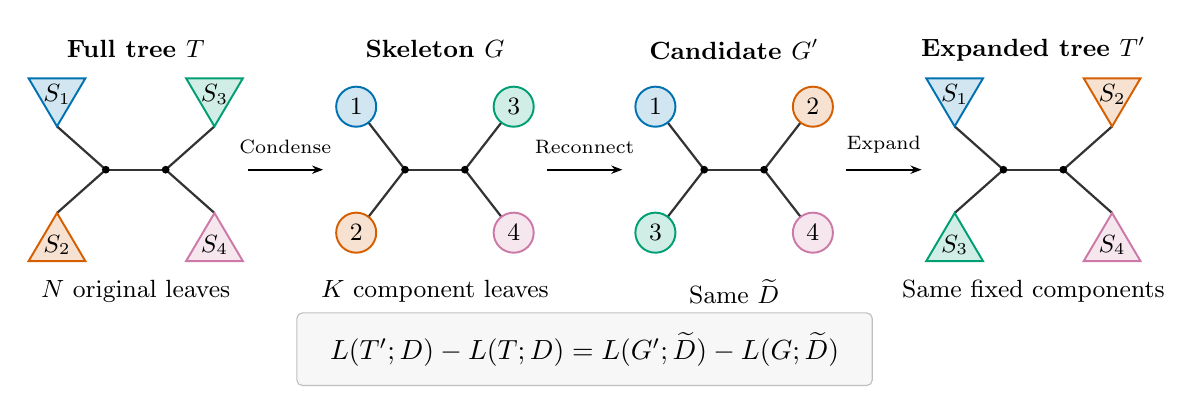
\begin{tikzpicture}[tree/.style={line width=.8pt,draw=black!80},
                   >={Stealth[length=4pt]}]
 \fullquartet{0}{1/compA}{2/compB}{3/compC}{4/compD}
 \skeleton{3.8}{1/compA}{2/compB}{3/compC}{4/compD}
 \skeleton{7.6}{1/compA}{3/compC}{2/compB}{4/compD}
 \fullquartet{11.4}{1/compA}{3/compC}{2/compB}{4/compD}

 \foreach \x/\name in {0/{Full tree $T$},3.8/{Skeleton $G$},
                        7.6/{Candidate $G'$},11.4/{Expanded tree $T'$}}
   \node[font=\small\bfseries] at (\x,1.53) {\name};

 \foreach \x/\name in {1.9/Condense,5.7/Reconnect,9.5/Expand}{
   \draw[->,line width=.7pt] (\x-.48,0)--(\x+.48,0);
   \node[font=\scriptsize,anchor=south] at (\x,.08) {\name};
 }
 \node[font=\small] at (0,-1.55) {$N$ original leaves};
 \node[font=\small] at (3.8,-1.55) {$K$ component leaves};
 \node[font=\small] at (7.6,-1.55) {Same $\widetilde D$};
 \node[font=\small] at (11.4,-1.55) {Same fixed components};

 \node[draw=black!25,rounded corners=2pt,fill=black!3,
       inner xsep=12pt,inner ysep=7pt,font=\normalsize]
   at (5.7,-2.28)
   {$L(T';D)-L(T;D)=L(G';\widetilde D)-L(G;\widetilde D)$};
\end{tikzpicture}
\end{document}
